% Options for packages loaded elsewhere
\PassOptionsToPackage{unicode}{hyperref}
\PassOptionsToPackage{hyphens}{url}
\PassOptionsToPackage{dvipsnames,svgnames,x11names}{xcolor}
%
\documentclass[
  letterpaper,
  DIV=11,
  numbers=noendperiod]{scrartcl}

\usepackage{amsmath,amssymb}
\usepackage{iftex}
\ifPDFTeX
  \usepackage[T1]{fontenc}
  \usepackage[utf8]{inputenc}
  \usepackage{textcomp} % provide euro and other symbols
\else % if luatex or xetex
  \usepackage{unicode-math}
  \defaultfontfeatures{Scale=MatchLowercase}
  \defaultfontfeatures[\rmfamily]{Ligatures=TeX,Scale=1}
\fi
\usepackage{lmodern}
\ifPDFTeX\else  
    % xetex/luatex font selection
\fi
% Use upquote if available, for straight quotes in verbatim environments
\IfFileExists{upquote.sty}{\usepackage{upquote}}{}
\IfFileExists{microtype.sty}{% use microtype if available
  \usepackage[]{microtype}
  \UseMicrotypeSet[protrusion]{basicmath} % disable protrusion for tt fonts
}{}
\makeatletter
\@ifundefined{KOMAClassName}{% if non-KOMA class
  \IfFileExists{parskip.sty}{%
    \usepackage{parskip}
  }{% else
    \setlength{\parindent}{0pt}
    \setlength{\parskip}{6pt plus 2pt minus 1pt}}
}{% if KOMA class
  \KOMAoptions{parskip=half}}
\makeatother
\usepackage{xcolor}
\usepackage[left=1in,right=1in,top=1in,bottom=1in]{geometry}
\setlength{\emergencystretch}{3em} % prevent overfull lines
\setcounter{secnumdepth}{-\maxdimen} % remove section numbering
% Make \paragraph and \subparagraph free-standing
\makeatletter
\ifx\paragraph\undefined\else
  \let\oldparagraph\paragraph
  \renewcommand{\paragraph}{
    \@ifstar
      \xxxParagraphStar
      \xxxParagraphNoStar
  }
  \newcommand{\xxxParagraphStar}[1]{\oldparagraph*{#1}\mbox{}}
  \newcommand{\xxxParagraphNoStar}[1]{\oldparagraph{#1}\mbox{}}
\fi
\ifx\subparagraph\undefined\else
  \let\oldsubparagraph\subparagraph
  \renewcommand{\subparagraph}{
    \@ifstar
      \xxxSubParagraphStar
      \xxxSubParagraphNoStar
  }
  \newcommand{\xxxSubParagraphStar}[1]{\oldsubparagraph*{#1}\mbox{}}
  \newcommand{\xxxSubParagraphNoStar}[1]{\oldsubparagraph{#1}\mbox{}}
\fi
\makeatother

\usepackage{color}
\usepackage{fancyvrb}
\newcommand{\VerbBar}{|}
\newcommand{\VERB}{\Verb[commandchars=\\\{\}]}
\DefineVerbatimEnvironment{Highlighting}{Verbatim}{commandchars=\\\{\}}
% Add ',fontsize=\small' for more characters per line
\usepackage{framed}
\definecolor{shadecolor}{RGB}{241,243,245}
\newenvironment{Shaded}{\begin{snugshade}}{\end{snugshade}}
\newcommand{\AlertTok}[1]{\textcolor[rgb]{0.68,0.00,0.00}{#1}}
\newcommand{\AnnotationTok}[1]{\textcolor[rgb]{0.37,0.37,0.37}{#1}}
\newcommand{\AttributeTok}[1]{\textcolor[rgb]{0.40,0.45,0.13}{#1}}
\newcommand{\BaseNTok}[1]{\textcolor[rgb]{0.68,0.00,0.00}{#1}}
\newcommand{\BuiltInTok}[1]{\textcolor[rgb]{0.00,0.23,0.31}{#1}}
\newcommand{\CharTok}[1]{\textcolor[rgb]{0.13,0.47,0.30}{#1}}
\newcommand{\CommentTok}[1]{\textcolor[rgb]{0.37,0.37,0.37}{#1}}
\newcommand{\CommentVarTok}[1]{\textcolor[rgb]{0.37,0.37,0.37}{\textit{#1}}}
\newcommand{\ConstantTok}[1]{\textcolor[rgb]{0.56,0.35,0.01}{#1}}
\newcommand{\ControlFlowTok}[1]{\textcolor[rgb]{0.00,0.23,0.31}{\textbf{#1}}}
\newcommand{\DataTypeTok}[1]{\textcolor[rgb]{0.68,0.00,0.00}{#1}}
\newcommand{\DecValTok}[1]{\textcolor[rgb]{0.68,0.00,0.00}{#1}}
\newcommand{\DocumentationTok}[1]{\textcolor[rgb]{0.37,0.37,0.37}{\textit{#1}}}
\newcommand{\ErrorTok}[1]{\textcolor[rgb]{0.68,0.00,0.00}{#1}}
\newcommand{\ExtensionTok}[1]{\textcolor[rgb]{0.00,0.23,0.31}{#1}}
\newcommand{\FloatTok}[1]{\textcolor[rgb]{0.68,0.00,0.00}{#1}}
\newcommand{\FunctionTok}[1]{\textcolor[rgb]{0.28,0.35,0.67}{#1}}
\newcommand{\ImportTok}[1]{\textcolor[rgb]{0.00,0.46,0.62}{#1}}
\newcommand{\InformationTok}[1]{\textcolor[rgb]{0.37,0.37,0.37}{#1}}
\newcommand{\KeywordTok}[1]{\textcolor[rgb]{0.00,0.23,0.31}{\textbf{#1}}}
\newcommand{\NormalTok}[1]{\textcolor[rgb]{0.00,0.23,0.31}{#1}}
\newcommand{\OperatorTok}[1]{\textcolor[rgb]{0.37,0.37,0.37}{#1}}
\newcommand{\OtherTok}[1]{\textcolor[rgb]{0.00,0.23,0.31}{#1}}
\newcommand{\PreprocessorTok}[1]{\textcolor[rgb]{0.68,0.00,0.00}{#1}}
\newcommand{\RegionMarkerTok}[1]{\textcolor[rgb]{0.00,0.23,0.31}{#1}}
\newcommand{\SpecialCharTok}[1]{\textcolor[rgb]{0.37,0.37,0.37}{#1}}
\newcommand{\SpecialStringTok}[1]{\textcolor[rgb]{0.13,0.47,0.30}{#1}}
\newcommand{\StringTok}[1]{\textcolor[rgb]{0.13,0.47,0.30}{#1}}
\newcommand{\VariableTok}[1]{\textcolor[rgb]{0.07,0.07,0.07}{#1}}
\newcommand{\VerbatimStringTok}[1]{\textcolor[rgb]{0.13,0.47,0.30}{#1}}
\newcommand{\WarningTok}[1]{\textcolor[rgb]{0.37,0.37,0.37}{\textit{#1}}}

\providecommand{\tightlist}{%
  \setlength{\itemsep}{0pt}\setlength{\parskip}{0pt}}\usepackage{longtable,booktabs,array}
\usepackage{calc} % for calculating minipage widths
% Correct order of tables after \paragraph or \subparagraph
\usepackage{etoolbox}
\makeatletter
\patchcmd\longtable{\par}{\if@noskipsec\mbox{}\fi\par}{}{}
\makeatother
% Allow footnotes in longtable head/foot
\IfFileExists{footnotehyper.sty}{\usepackage{footnotehyper}}{\usepackage{footnote}}
\makesavenoteenv{longtable}
\usepackage{graphicx}
\makeatletter
\def\maxwidth{\ifdim\Gin@nat@width>\linewidth\linewidth\else\Gin@nat@width\fi}
\def\maxheight{\ifdim\Gin@nat@height>\textheight\textheight\else\Gin@nat@height\fi}
\makeatother
% Scale images if necessary, so that they will not overflow the page
% margins by default, and it is still possible to overwrite the defaults
% using explicit options in \includegraphics[width, height, ...]{}
\setkeys{Gin}{width=\maxwidth,height=\maxheight,keepaspectratio}
% Set default figure placement to htbp
\makeatletter
\def\fps@figure{htbp}
\makeatother

\usepackage{booktabs}
\usepackage{longtable}
\usepackage{array}
\usepackage{multirow}
\usepackage{wrapfig}
\usepackage{float}
\usepackage{colortbl}
\usepackage{pdflscape}
\usepackage{tabu}
\usepackage{threeparttable}
\usepackage{threeparttablex}
\usepackage[normalem]{ulem}
\usepackage{makecell}
\usepackage{xcolor}
\usepackage{fvextra}
\DefineVerbatimEnvironment{Highlighting}{Verbatim}{breaklines,commandchars=\\\{\}}
\DefineVerbatimEnvironment{OutputCode}{Verbatim}{breaklines,commandchars=\\\{\}}
\KOMAoption{captions}{tableheading}
\makeatletter
\@ifpackageloaded{caption}{}{\usepackage{caption}}
\AtBeginDocument{%
\ifdefined\contentsname
  \renewcommand*\contentsname{Table of contents}
\else
  \newcommand\contentsname{Table of contents}
\fi
\ifdefined\listfigurename
  \renewcommand*\listfigurename{List of Figures}
\else
  \newcommand\listfigurename{List of Figures}
\fi
\ifdefined\listtablename
  \renewcommand*\listtablename{List of Tables}
\else
  \newcommand\listtablename{List of Tables}
\fi
\ifdefined\figurename
  \renewcommand*\figurename{Figure}
\else
  \newcommand\figurename{Figure}
\fi
\ifdefined\tablename
  \renewcommand*\tablename{Table}
\else
  \newcommand\tablename{Table}
\fi
}
\@ifpackageloaded{float}{}{\usepackage{float}}
\floatstyle{ruled}
\@ifundefined{c@chapter}{\newfloat{codelisting}{h}{lop}}{\newfloat{codelisting}{h}{lop}[chapter]}
\floatname{codelisting}{Listing}
\newcommand*\listoflistings{\listof{codelisting}{List of Listings}}
\makeatother
\makeatletter
\makeatother
\makeatletter
\@ifpackageloaded{caption}{}{\usepackage{caption}}
\@ifpackageloaded{subcaption}{}{\usepackage{subcaption}}
\makeatother

\ifLuaTeX
  \usepackage{selnolig}  % disable illegal ligatures
\fi
\usepackage{bookmark}

\IfFileExists{xurl.sty}{\usepackage{xurl}}{} % add URL line breaks if available
\urlstyle{same} % disable monospaced font for URLs
\hypersetup{
  pdftitle={Case Study 1: Your Informative Title Here},
  pdfauthor={Miya Dang, Mia Tran},
  colorlinks=true,
  linkcolor={blue},
  filecolor={Maroon},
  citecolor={Blue},
  urlcolor={Blue},
  pdfcreator={LaTeX via pandoc}}


\title{Case Study 1: Your Informative Title Here}
\author{Miya Dang, Mia Tran}
\date{2025-03-05}

\begin{document}
\maketitle


\subsubsection{Introduction}\label{introduction}

The U.S. presidential election in 2000 between George W. Bush and Al
Gore was one of the closest in history, with its final outcome dependent
on the results in the state of Florida. Ultimately, Bush secured victory
by a margin of fewer than 400 votes. However, Democratic voters in Palm
Beach County argued that a confusing ``butterfly'' ballot layout led
them to mistakenly vote for Reform Party candidate Pat Buchanan instead
of Gore. This claim was supported by evidence showing that Buchanan
received an unusually high percentage of votes in the county, along with
a significant number of discarded ballots where voters had marked two
choices.

In this case study, we will model the relationship between Bush and
Buchanan votes in 2000 across Florida (excluding Palm Beach County to
assess its anomaly) to answer two questions:

\begin{itemize}
\tightlist
\item
  \emph{Was the number of votes for Buchanan in Palm Beach County
  statistically unusual compared to other Florida counties?}
\item
  \emph{What is the estimated number of votes intended for Gore but cast
  for Buchanan in Palm Beach County?}
\end{itemize}

\subsubsection{Data Description}\label{data-description}

The dataset contains the vote counts for Buchanan and Bush in 2000
across all 67 counties in Florida.

\textbf{Summary Statistics:}

\begin{verbatim}
    Bush2000       Buchanan2000   
 Min.   :  1316   Min.   :   9.0  
 1st Qu.:  4746   1st Qu.:  46.5  
 Median : 20196   Median : 114.0  
 Mean   : 43356   Mean   : 258.5  
 3rd Qu.: 56542   3rd Qu.: 285.5  
 Max.   :289456   Max.   :3407.0  
\end{verbatim}

\begin{itemize}
\item
  Summary statistics indicate that, overall, Bush received significantly
  higher votes than Buchanan.
\item
  Both variables have means much higher than their medians, indicating a
  strong right skew. This suggests that most counties had relatively low
  vote counts, while a small number had exceptionally high vote counts.
\item
  The maximum number of Buchanan votes was 3,407, far exceeding the
  third quantile of 285.5. This vote count came from Palm Beach County,
  suggesting that it is an outlier.
\end{itemize}

\textbf{Accompanying Graph:}

The scatterplot below visualizes the relationship between Bush votes
(x-axis) and Buchanan votes (y-axis) for all 67 counties:

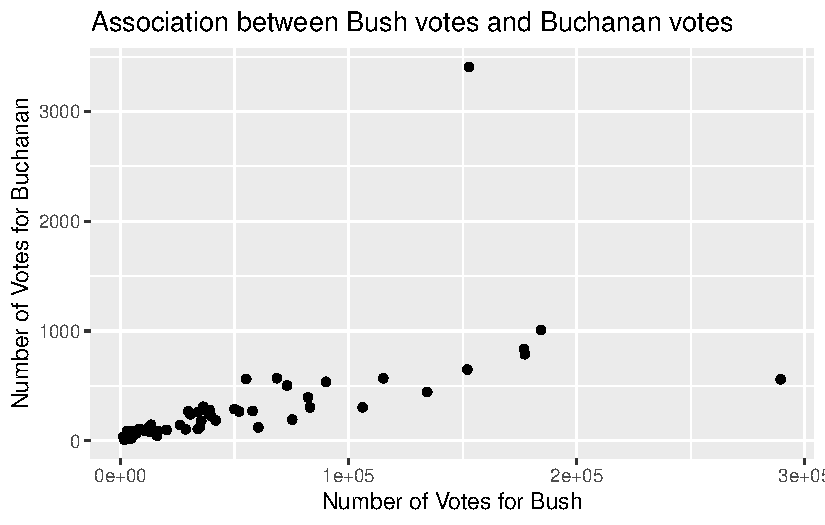
\includegraphics{SDS-291-case-study-1_files/figure-pdf/unnamed-chunk-3-1.pdf}

There is a general positive trend, as counties with more Bush votes also
tended to have more Buchanan votes. Palm Beach County (the mark on the
top of the graph) is a notable outlier with unexpectedly high Buchanan
votes (3,407).

\subsubsection{Modeling Process and
Results}\label{modeling-process-and-results}

Let \(Buchanan\) denote the votes for Buchanan in Palm Beach County and
\(Bush\) denote the the votes for Bush in Palm Beach County. Our final
linear regression model is:
\[E[log(Buchanan) | log(Bush)] = \beta_0 + \beta_1\left(Bush\right).\]

The prediction interval is \([365, 831]\). We are 95\% confident that
the votes for Buchanan when there are 152846 votes for Bush will fall
between 365 votes and 831 votes.

Buchanan's real vote from Palm Beach County in 2000 election is 3407
votes. Compared to the prediction interval above, we can calculate that
an estimate for the likely number of votes intended for Gore but cast
for Buchanan in Palm Beach County falls between \([2576, 3042]\).

\subsubsection{Summary and Conclusions}\label{summary-and-conclusions}

\textbf{Key Findings}

\begin{itemize}
\item
  The Buchanan vote count in Palm Beach County during the 2000 election
  was statistically unusual.
\item
  An estimated 2,576 to 3,042 votes intended for Gore were likely
  miscast for Buchanan.
\item
  These results suggest that the ballot design may have altered the
  election outcome. Given that Gore lost Florida by fewer than 400
  votes, the potential miscast votes in Palm Beach County alone far
  exceed this margin.
\end{itemize}

\textbf{Limitations}

\begin{itemize}
\item
  The log-log transformation assumes a multiplicative relationship
  between Bush and Buchanan votes. While this improved linearity,
  residual diagnostics revealed mild heteroscedasticity and a slightly
  left-skewed residual distribution. These imply that the prediction
  interval may underestimate uncertainty, particularly for counties with
  high Bush vote count like Palm Beach.
\item
  The model assumes that voter behavior is similar across all counties.
  However, many other factors could contribute to regional differences
  between voter behavior, such as candidate campaigns or other
  demographic factors.
\item
  The analysis demonstrate association and not causation. Further
  investigation would be necessary to definitively prove that the
  butterfly ballot caused the excess Buchanan votes.
\end{itemize}

\subsection{R Appendix}\label{r-appendix}

\begin{Shaded}
\begin{Highlighting}[]
\CommentTok{\# Loading necessary packages}
\FunctionTok{library}\NormalTok{(tidyverse)}
\FunctionTok{library}\NormalTok{(Sleuth2)}
\FunctionTok{library}\NormalTok{(broom)        }
\FunctionTok{library}\NormalTok{(kableExtra)   }

\CommentTok{\# Loading the data for case study one}
\NormalTok{election }\OtherTok{\textless{}{-}}\NormalTok{ Sleuth2}\SpecialCharTok{::}\NormalTok{ex0825}

\CommentTok{\# Summary statistics}
\FunctionTok{summary}\NormalTok{(election }\SpecialCharTok{\%\textgreater{}\%} \FunctionTok{select}\NormalTok{(Bush2000, Buchanan2000))}
\end{Highlighting}
\end{Shaded}

\begin{verbatim}
    Bush2000       Buchanan2000   
 Min.   :  1316   Min.   :   9.0  
 1st Qu.:  4746   1st Qu.:  46.5  
 Median : 20196   Median : 114.0  
 Mean   : 43356   Mean   : 258.5  
 3rd Qu.: 56542   3rd Qu.: 285.5  
 Max.   :289456   Max.   :3407.0  
\end{verbatim}

\begin{Shaded}
\begin{Highlighting}[]
\CommentTok{\# Creating a scatterplot for the relationship between Bush and Buchanan votes}
\NormalTok{election }\SpecialCharTok{|\textgreater{}}
  \FunctionTok{ggplot}\NormalTok{(}\FunctionTok{aes}\NormalTok{(}\AttributeTok{x =}\NormalTok{ Bush2000,}
             \AttributeTok{y =}\NormalTok{ Buchanan2000)) }\SpecialCharTok{+}
  \FunctionTok{geom\_point}\NormalTok{() }\SpecialCharTok{+}
  \FunctionTok{ggtitle}\NormalTok{(}\StringTok{"Association between Bush votes and Buchanan votes"}\NormalTok{)}
\end{Highlighting}
\end{Shaded}

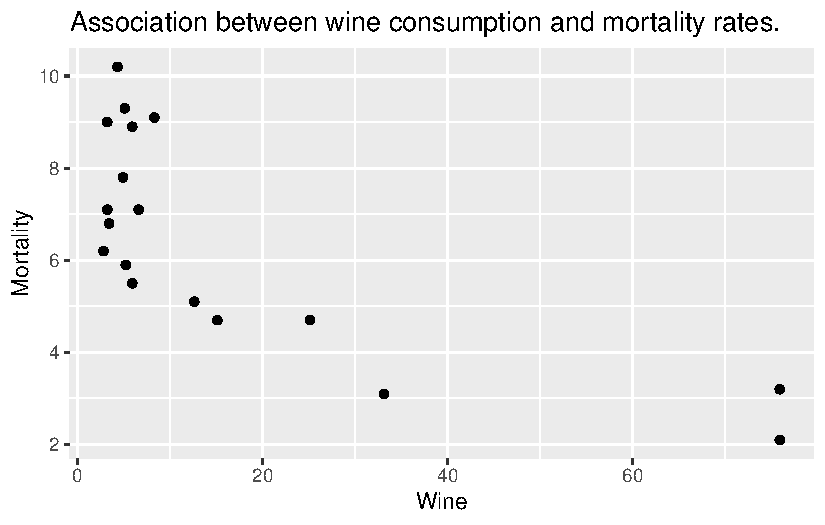
\includegraphics{SDS-291-case-study-1_files/figure-pdf/unnamed-chunk-4-1.pdf}

\begin{Shaded}
\begin{Highlighting}[]
\CommentTok{\# Creating a second dataset with Palm Beach County excluded}
\NormalTok{election\_wo\_pb }\OtherTok{\textless{}{-}}\NormalTok{ election }\SpecialCharTok{|\textgreater{}}
  \FunctionTok{filter}\NormalTok{(County }\SpecialCharTok{!=} \StringTok{"Palm Beach"}\NormalTok{)}

\CommentTok{\# Fitting and summarizing the regression line for mean Buchanan votes }
\CommentTok{\# as a function of Bush votes}
\NormalTok{election\_lm }\OtherTok{\textless{}{-}} \FunctionTok{lm}\NormalTok{(Buchanan2000 }\SpecialCharTok{\textasciitilde{}}\NormalTok{ Bush2000, }\AttributeTok{data =}\NormalTok{ election\_wo\_pb)}
\FunctionTok{summary}\NormalTok{(election\_lm)}\SpecialCharTok{$}\NormalTok{coefficients}
\end{Highlighting}
\end{Shaded}

\begin{verbatim}
                Estimate   Std. Error   t value     Pr(>|t|)
(Intercept) 65.573496362 1.733043e+01  3.783721 3.427131e-04
Bush2000     0.003481898 2.500903e-04 13.922562 4.916245e-21
\end{verbatim}

\begin{Shaded}
\begin{Highlighting}[]
\NormalTok{election\_lm\_table }\OtherTok{\textless{}{-}} \FunctionTok{summary}\NormalTok{(election\_lm)}\SpecialCharTok{$}\NormalTok{coefficients}

\CommentTok{\# Creating the table summarizing the estimated coefficients of the model }
\CommentTok{\# and their corresponding standard errors}
\NormalTok{election\_lm\_table }\SpecialCharTok{|\textgreater{}} \FunctionTok{kbl}\NormalTok{(}\AttributeTok{col.names =} \FunctionTok{c}\NormalTok{(}\StringTok{"Estimate"}\NormalTok{, }\StringTok{"Std. Error"}\NormalTok{,}
                                       \StringTok{"t value"}\NormalTok{, }\StringTok{"Pr(\textgreater{}|t|)"}\NormalTok{), }
                         \AttributeTok{align =} \StringTok{"c"}\NormalTok{,}
                         \AttributeTok{booktabs =}\NormalTok{ T,}
                         \AttributeTok{linesep=}\StringTok{""}\NormalTok{,}
                         \AttributeTok{digits =} \FunctionTok{c}\NormalTok{(}\DecValTok{4}\NormalTok{, }\DecValTok{4}\NormalTok{, }\DecValTok{4}\NormalTok{, }\DecValTok{4}\NormalTok{)) }\SpecialCharTok{|\textgreater{}}
  \FunctionTok{kable\_classic}\NormalTok{(}\AttributeTok{full\_width =}\NormalTok{ F, }\AttributeTok{latex\_options =} \FunctionTok{c}\NormalTok{(}\StringTok{"HOLD\_position"}\NormalTok{))}
\end{Highlighting}
\end{Shaded}

\begin{table}[H]
\centering
\begin{tabular}[t]{lcccc}
\toprule
  & Estimate & Std. Error & t value & Pr(>|t|)\\
\midrule
(Intercept) & 65.5735 & 17.3304 & 3.7837 & 3e-04\\
Bush2000 & 0.0035 & 0.0003 & 13.9226 & 0e+00\\
\bottomrule
\end{tabular}
\end{table}

\begin{Shaded}
\begin{Highlighting}[]
\CommentTok{\# Creating the residuals{-}fitted plot to check }
\CommentTok{\# Linearity and Equal Variance for the election model}
\NormalTok{election\_lm }\SpecialCharTok{|\textgreater{}}
  \FunctionTok{augment}\NormalTok{() }\SpecialCharTok{|\textgreater{}}
  \FunctionTok{ggplot}\NormalTok{(}\FunctionTok{aes}\NormalTok{(}\AttributeTok{x =}\NormalTok{ .fitted, }\AttributeTok{y =}\NormalTok{ .resid)) }\SpecialCharTok{+}
  \FunctionTok{geom\_point}\NormalTok{() }\SpecialCharTok{+}
  \FunctionTok{geom\_hline}\NormalTok{(}\AttributeTok{yintercept =} \DecValTok{0}\NormalTok{, }\AttributeTok{col =} \StringTok{"red"}\NormalTok{) }\SpecialCharTok{+}
  \FunctionTok{xlab}\NormalTok{(}\StringTok{"Fitted Values"}\NormalTok{) }\SpecialCharTok{+}
  \FunctionTok{ylab}\NormalTok{(}\StringTok{"Residuals"}\NormalTok{) }\SpecialCharTok{+}
  \FunctionTok{theme\_bw}\NormalTok{()}
\end{Highlighting}
\end{Shaded}

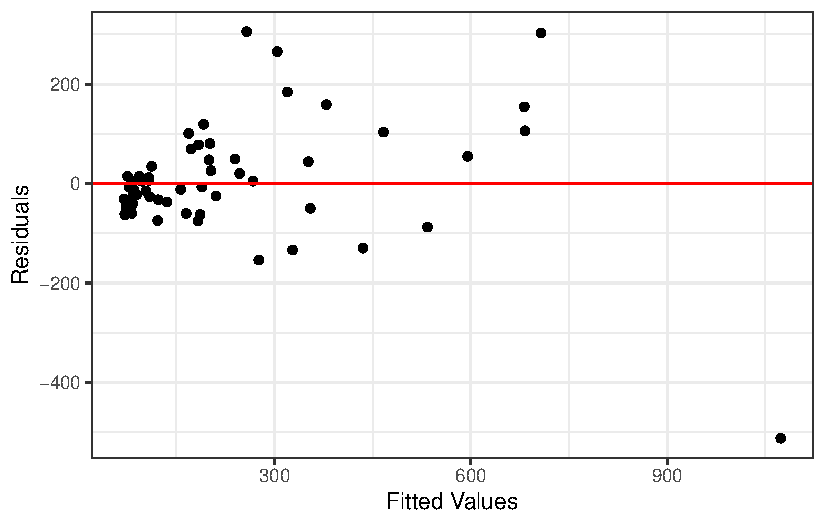
\includegraphics{SDS-291-case-study-1_files/figure-pdf/unnamed-chunk-4-2.pdf}

\begin{Shaded}
\begin{Highlighting}[]
\CommentTok{\# Creating the Q{-}Q plot as check Normality for the election model}
\NormalTok{election\_lm }\SpecialCharTok{|\textgreater{}}
  \FunctionTok{augment}\NormalTok{() }\SpecialCharTok{|\textgreater{}}
  \FunctionTok{ggplot}\NormalTok{(}\FunctionTok{aes}\NormalTok{(}\AttributeTok{sample =}\NormalTok{ .resid)) }\SpecialCharTok{+}
  \FunctionTok{geom\_qq}\NormalTok{() }\SpecialCharTok{+}
  \FunctionTok{geom\_qq\_line}\NormalTok{(}\AttributeTok{col =} \StringTok{"blue"}\NormalTok{) }\SpecialCharTok{+}
  \FunctionTok{xlab}\NormalTok{(}\StringTok{"Theoretical Quantiles"}\NormalTok{) }\SpecialCharTok{+}
  \FunctionTok{ylab}\NormalTok{(}\StringTok{"Sample Quantiles"}\NormalTok{) }\SpecialCharTok{+}
  \FunctionTok{theme\_bw}\NormalTok{()}
\end{Highlighting}
\end{Shaded}

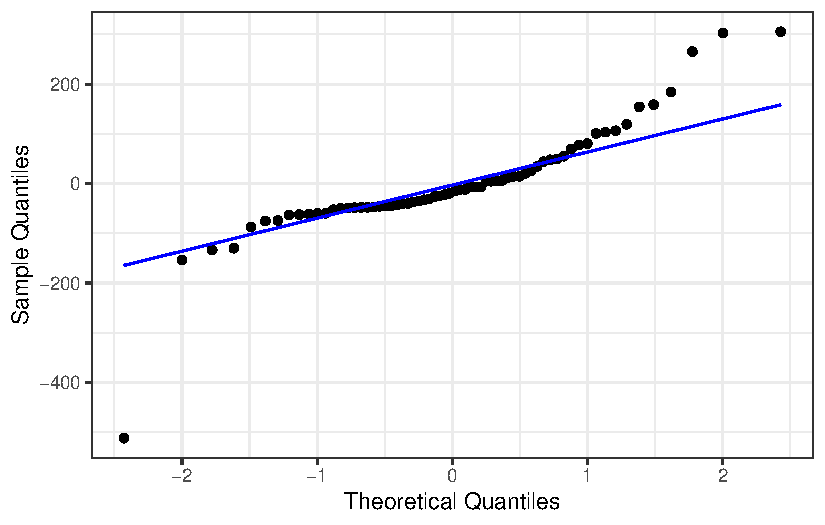
\includegraphics{SDS-291-case-study-1_files/figure-pdf/unnamed-chunk-4-3.pdf}

\begin{Shaded}
\begin{Highlighting}[]
\CommentTok{\#Transformation}
\NormalTok{transformed\_election\_lm }\OtherTok{\textless{}{-}} \FunctionTok{lm}\NormalTok{(}\FunctionTok{log}\NormalTok{(Buchanan2000) }\SpecialCharTok{\textasciitilde{}} \FunctionTok{log}\NormalTok{(Bush2000), election\_wo\_pb)}

\CommentTok{\# Creating the residuals{-}fitted plot to check }
\CommentTok{\# Linearity and Equal Variance for the transformed election model}
\NormalTok{transformed\_election\_lm }\SpecialCharTok{|\textgreater{}}
  \FunctionTok{augment}\NormalTok{() }\SpecialCharTok{|\textgreater{}}
  \FunctionTok{ggplot}\NormalTok{(}\FunctionTok{aes}\NormalTok{(}\AttributeTok{x =}\NormalTok{ .fitted, }\AttributeTok{y =}\NormalTok{ .resid)) }\SpecialCharTok{+}
  \FunctionTok{geom\_point}\NormalTok{() }\SpecialCharTok{+}
  \FunctionTok{geom\_hline}\NormalTok{(}\AttributeTok{yintercept =} \DecValTok{0}\NormalTok{, }\AttributeTok{col =} \StringTok{"red"}\NormalTok{) }\SpecialCharTok{+}
  \FunctionTok{xlab}\NormalTok{(}\StringTok{"Fitted Values"}\NormalTok{) }\SpecialCharTok{+}
  \FunctionTok{ylab}\NormalTok{(}\StringTok{"Residuals"}\NormalTok{) }\SpecialCharTok{+}
  \FunctionTok{theme\_bw}\NormalTok{()}
\end{Highlighting}
\end{Shaded}

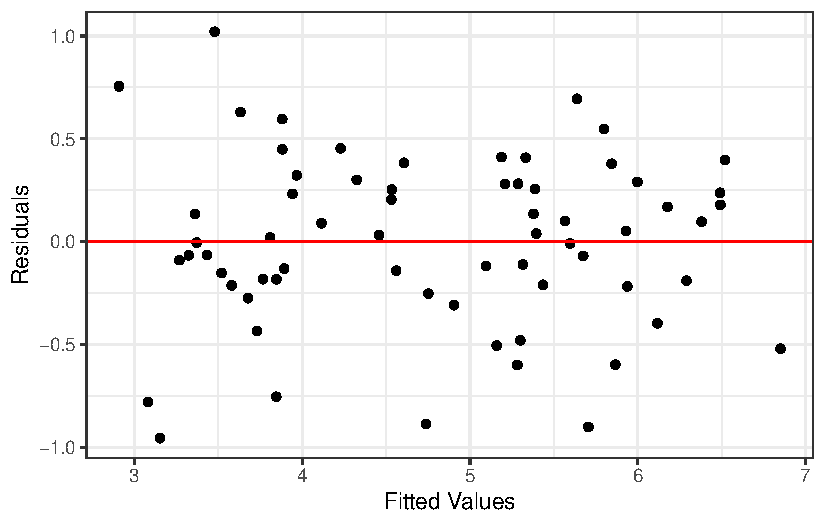
\includegraphics{SDS-291-case-study-1_files/figure-pdf/unnamed-chunk-4-4.pdf}

\begin{Shaded}
\begin{Highlighting}[]
\CommentTok{\# Creating the Q{-}Q plot as check Normality for the transformed election model}
\NormalTok{transformed\_election\_lm }\SpecialCharTok{|\textgreater{}}
  \FunctionTok{augment}\NormalTok{() }\SpecialCharTok{|\textgreater{}}
  \FunctionTok{ggplot}\NormalTok{(}\FunctionTok{aes}\NormalTok{(}\AttributeTok{sample =}\NormalTok{ .resid)) }\SpecialCharTok{+}
  \FunctionTok{geom\_qq}\NormalTok{() }\SpecialCharTok{+}
  \FunctionTok{geom\_qq\_line}\NormalTok{(}\AttributeTok{col =} \StringTok{"blue"}\NormalTok{) }\SpecialCharTok{+}
  \FunctionTok{xlab}\NormalTok{(}\StringTok{"Theoretical Quantiles"}\NormalTok{) }\SpecialCharTok{+}
  \FunctionTok{ylab}\NormalTok{(}\StringTok{"Sample Quantiles"}\NormalTok{) }\SpecialCharTok{+}
  \FunctionTok{theme\_bw}\NormalTok{()}
\end{Highlighting}
\end{Shaded}

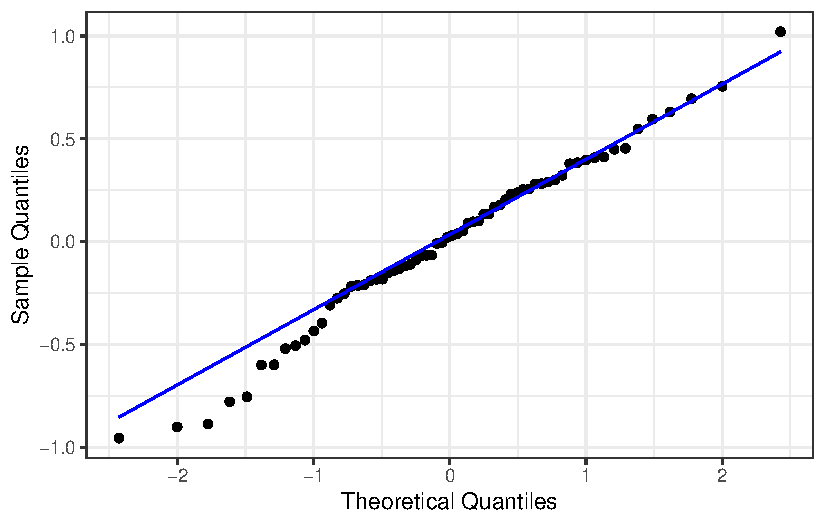
\includegraphics{SDS-291-case-study-1_files/figure-pdf/unnamed-chunk-4-5.pdf}

\begin{Shaded}
\begin{Highlighting}[]
\CommentTok{\# Filter the original dataset to only Palm Beach Country}
\CommentTok{\# to create prediction interval}
\NormalTok{election\_pb }\OtherTok{\textless{}{-}}\NormalTok{ election }\SpecialCharTok{|\textgreater{}} \FunctionTok{filter}\NormalTok{(County }\SpecialCharTok{==} \StringTok{"Palm Beach"}\NormalTok{)}

\CommentTok{\# Creating a 95\% prediction interval for the number of}
\CommentTok{\# predicted Buchanan votes in Palm Beach County}
\CommentTok{\# after knowing the votes for Bush from Palm Beach County}
\NormalTok{new\_election }\OtherTok{\textless{}{-}} \FunctionTok{data.frame}\NormalTok{(}\AttributeTok{Bush2000 =} \DecValTok{152846}\NormalTok{)}
\NormalTok{election\_lm }\SpecialCharTok{|\textgreater{}}
  \FunctionTok{augment}\NormalTok{(}\AttributeTok{newdata =}\NormalTok{ new\_election,}
          \AttributeTok{interval =} \StringTok{"prediction"}\NormalTok{,}
          \AttributeTok{conf.level =} \FloatTok{0.95}\NormalTok{)}
\end{Highlighting}
\end{Shaded}

\begin{verbatim}
# A tibble: 1 x 4
  Bush2000 .fitted .lower .upper
     <dbl>   <dbl>  <dbl>  <dbl>
1   152846    598.   365.   831.
\end{verbatim}




\end{document}
